\documentclass[12ampt]{article}
\setlength\parindent{0pt}
\usepackage{fullpage}
\usepackage{amsmath}
\usepackage{graphicx}
\setlength{\parskip}{4mm}
\def\LL{\left\langle}   % left angle bracket
\def\RR{\right\rangle}  % right angle bracket
\def\LP{\left(}         % left parenthesis
\def\RP{\right)}        % right parenthesis
\def\LB{\left\{}        % left curly bracket
\def\RB{\right\}}       % right curly bracket
\def\PAR#1#2{ {{\partial #1}\over{\partial #2}} }
\def\PARTWO#1#2{ {{\partial^2 #1}\over{\partial #2}^2} }
\def\PARTWOMIX#1#2#3{ {{\partial^2 #1}\over{\partial #2 \partial #3}} }
\newcommand{\BC}{\begin{center}}
\newcommand{\EC}{\end{center}}
\newcommand{\BE}{\begin{displaymath}}
\newcommand{\EE}{\end{displaymath}}
\newcommand{\BNE}{\begin{equation}}
\newcommand{\ENE}{\end{equation}}
\newcommand{\BEA}{\begin{eqnarray}}
\newcommand{\EEA}{\nonumber\end{eqnarray}}
\newcommand{\EL}{\nonumber\\}
\newcommand{\la}[1]{\label{#1}}
\newcommand{\ie}{{\em i.e.\ }}
\newcommand{\eg}{{\em e.\,g.\ }}
\newcommand{\cf}{cf.\ }
\newcommand{\etc}{etc.\ }
\newcommand{\Tr}{{\rm tr}}
\newcommand{\etal}{{\it et al.}}
\newcommand{\OL}[1]{\overline{#1}\ } % overline
\newcommand{\OLL}[1]{\overline{\overline{#1}}\ } % double overline
\newcommand{\OON}{\frac{1}{N}} % "one over N"
\newcommand{\OOX}[1]{\frac{1}{#1}} % "one over X"



\begin{document}
\Large
\centerline{\sc{Notes on numerical solution of differential equations}}
\normalsize

Some definitions, for those who don't know:

\begin{itemize}
\item A ``differential equation'' is any equation that relates a thing to its 
derivatives. For instance, Newton's second law of motion for a mass bouncing
on a string can be written
$-kx = m \PARTWO{x}{t}$, where I've put in Hooke's law for the force.

\item A ``system of differential equations'' is a group of equations 
that relate a bunch of things to their derivatives.

\item A ``first-order differential equation'' is one involving only first derivatives.

\item A ``second-order differential equation'' involves second derivatives.

\end{itemize}

A great many physics phenomena are described by (systems of) differential equations, so we need a way to solve them numerically. In our class, we're going to focus on time-variation problems of the following form:

{\bf Given the initial state of some system $y$, and the differential equation(s) that tell us how y changes with time, figure out what the system y looks like for all future times -- that is, find $y(t)$}.

For instance, we are very interested in computing the motions of objects, 
the evolution of electromagnetic fields, 
the propagation of heat, and so on, 
and these techniques give us a way to study that.

In general, these situations often take the form of a set of coupled second-order differential equations. 
However, such a situation can be reduced to a set of 
first-order DE's. So, in these notes I will build up the general case in three steps:

\begin{itemize}
  \item{A single first-order DE: the cooling cup of tea}
  \item{A single second-order DE: the swinging pendulum} 
  \item{Many second-order DE's: celestial motion}
\end{itemize}

\section{Euler's method for a single first-order DE}

Throughout I will use time as the independent variable, since this is usually the case we care about. However, everything works the same if some other 
coordinate is the independent variable.

A first-order differential equation has the form

\begin{equation}
  \PAR{y}{t} = f(y,t)
\end{equation}

where $y$ is a generic dependent variable and 
$f(y,t)$ gives its rate of change over time as a function of its value (and, sometimes, the time). Note the notation: $f$ here is not an arbitrary function, but 
the {\it specific function that tells you how fast $y$ changes}.
A specific example is 
Newton's law of cooling

\begin{equation}
  \PAR{T}{t} = f(t) = -k(T-T_a)
\end{equation}

which is the first problem you'll be solving. In words, it just says that 
{\bf an object cools at a rate proportional to the difference in temperature between
it and the room around it.}

This is the same behavior as you get from a charging/discharging capacitor (in 
electronics), incidentally. It behaves like this:

\BC
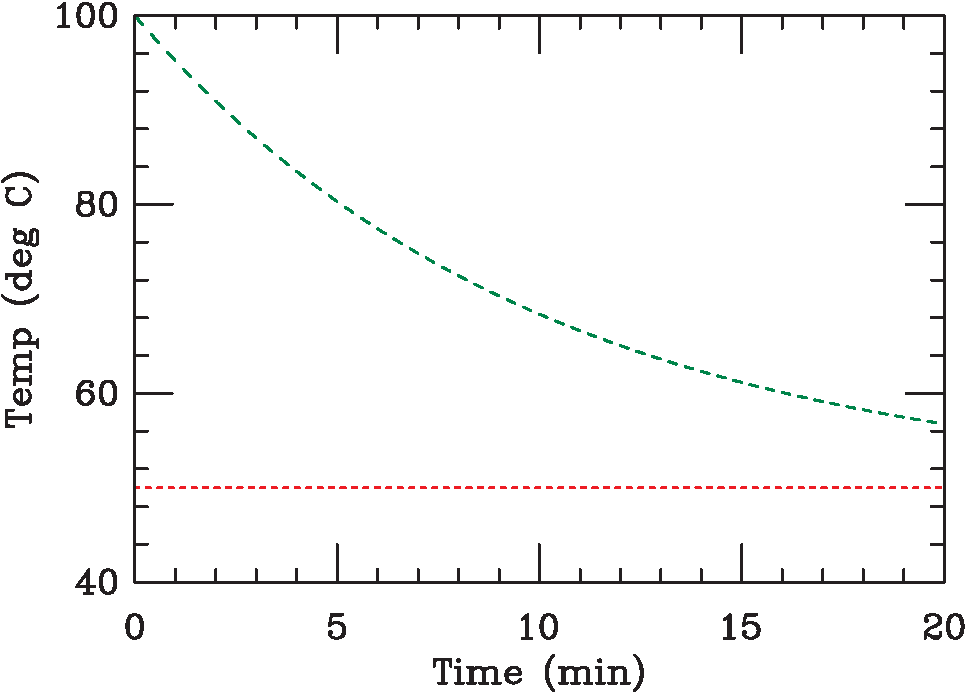
\includegraphics[width=0.5\textwidth]{cooling-intro-crop.pdf} \\
\scriptsize \it The behavior of a cooling thermos of tea (in a very hot room!) 
The green plot gives the temperature of the tea; the red line represents the 
ambient temperature of $50^\circ$ C (perhaps you're in Arizona in June, or the 
Physics Clinic in April!)
\EC

We need to figure out how to make a computer calculate this. The solution, as 
with most things in computational physics, involves {\it thinking about how you
would get a bunch of middle-schoolers with calculators to do it}, then simply 
telling the computer to do that.

Let's make a table. For illustration, I'll use $k=0.5 {\rm min}^{-1}$, with
$T_a=50$ and $T_0=100$ -- that is, we're starting with tea at 100 degrees that is
cooling down in a room that is 50 degrees.

\begin{tabular}{|c | c | c |}
\hline
Time (min) & Temp (C) & Slope: $\PAR{T}{t}$ \\
\hline
0 & 100 & \\
\hline
1 & &  \\
\hline
2 & &  \\
\hline
3 & &  \\
\hline
4 & &  \\
\hline
5 & &  \\
\hline
\end{tabular}

Our job is to fill in all the missing temperatures, using the only information we
have, the differential equation $$\PAR{T}{t}=-k(T-T_a).$$

This equation tells us the slope of the curve, given the current temperature $T$;
it comes out to $(100-50) \times 0.5$ = 25 degrees per minute.

I can show what I know now both in tabular form and as a graph:

\begin{minipage}{0.5\textwidth}
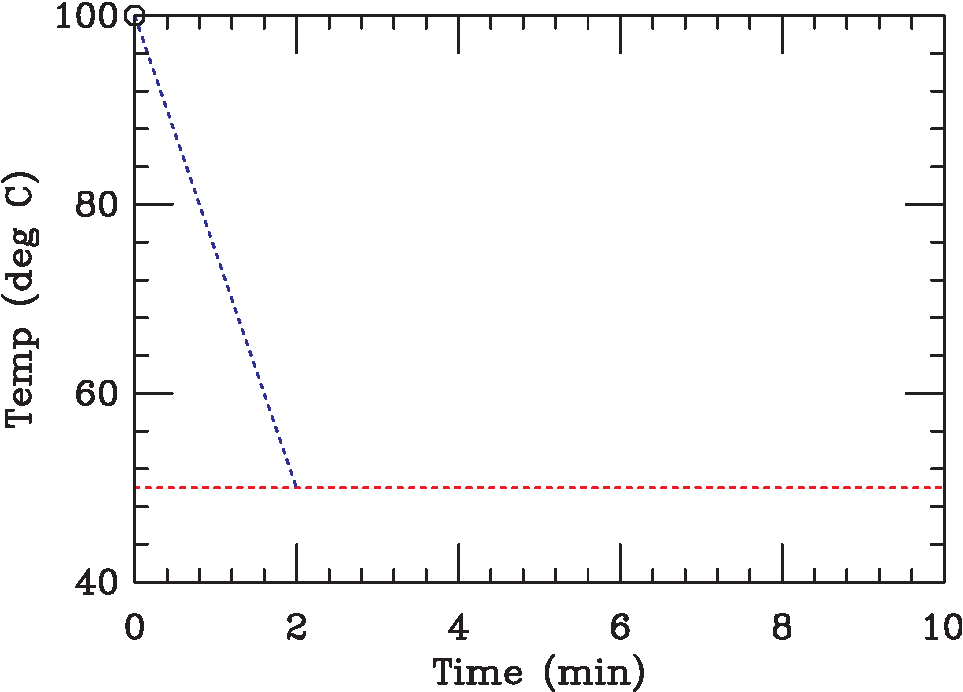
\includegraphics[width=0.9\textwidth]{fig0-crop.pdf}
\end{minipage}
\begin{minipage}{0.5\textwidth}
\begin{tabular}{|c | c | c |}
\hline
Time (min) & Temp (C) & Slope: $\PAR{T}{t}$ \\
\hline
0 & 100 & -25 \\
\hline
1 & &  \\
\hline
2 & &  \\
\hline
3 & &  \\
\hline
4 & &  \\
\hline
5 & &  \\
\hline
\end{tabular}
\end{minipage}

Here the black circle at $(t=0,T=100)$ indicates that I know the temperature is 
100 degrees at $t=0$; the blue dotted line shows my knowledge of the slope at this
point. 

Well, if I need to estimate the temperature after 1 minute, and I know the tea
is cooling at 25 degrees per minute, then I should just guess that the $T(1) = 
100 - 25 =75$ degrees. Graphically, what I'm doing is evaluating the slope at 
$(t=0, T=100)$ and following that down to $t=1$. 

\begin{minipage}{0.5\textwidth}
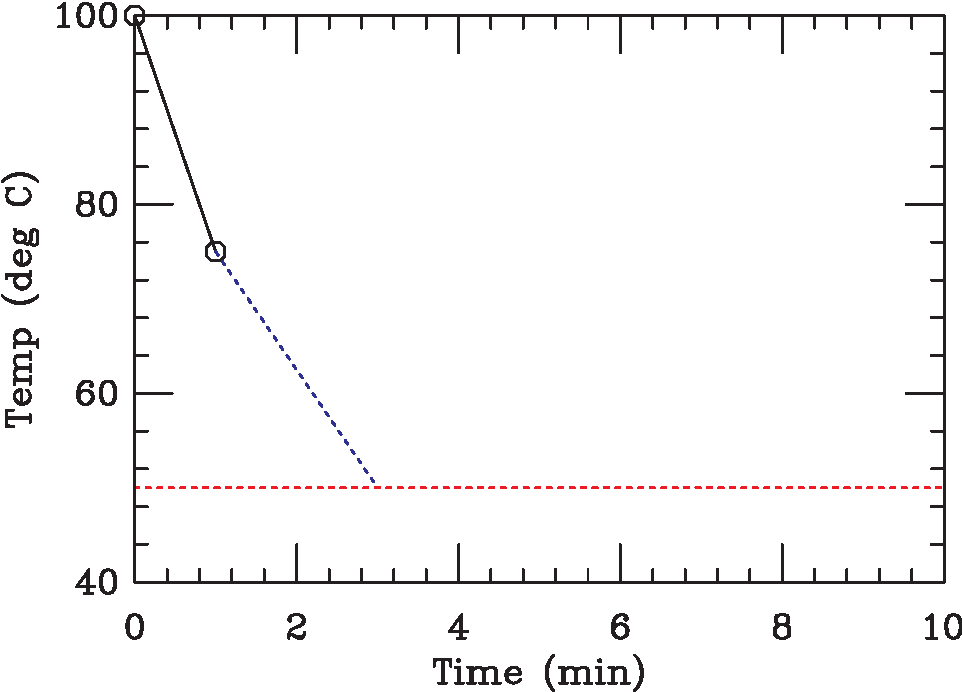
\includegraphics[width=0.9\textwidth]{fig1-crop.pdf}
\end{minipage}
\begin{minipage}{0.5\textwidth}
\begin{tabular}{|c | c | c |}
\hline
Time (min) & Temp (C) & Slope: $\PAR{T}{t}$ \\
\hline
0 & 100 & -25 \\
\hline
1 & 75 &  -12.5\\
\hline
2 & &  \\
\hline
3 & &  \\
\hline
4 & &  \\
\hline
5 & &  \\
\hline
\end{tabular}
\end{minipage}

Now I have some new information on both my table and graph: the point 
$(t=1,T=75)$, and the ability to calculate that the slope here is $-12.5$ degrees
per minute. That's reflected in both the chart and the graph above. 

You should be able to see how this goes at this point: we figure out the current
slope from the current temperature, and then use the current temperature and 
that slope to estimate the next temperature. Taking more steps we get:


\begin{minipage}{0.5\textwidth}
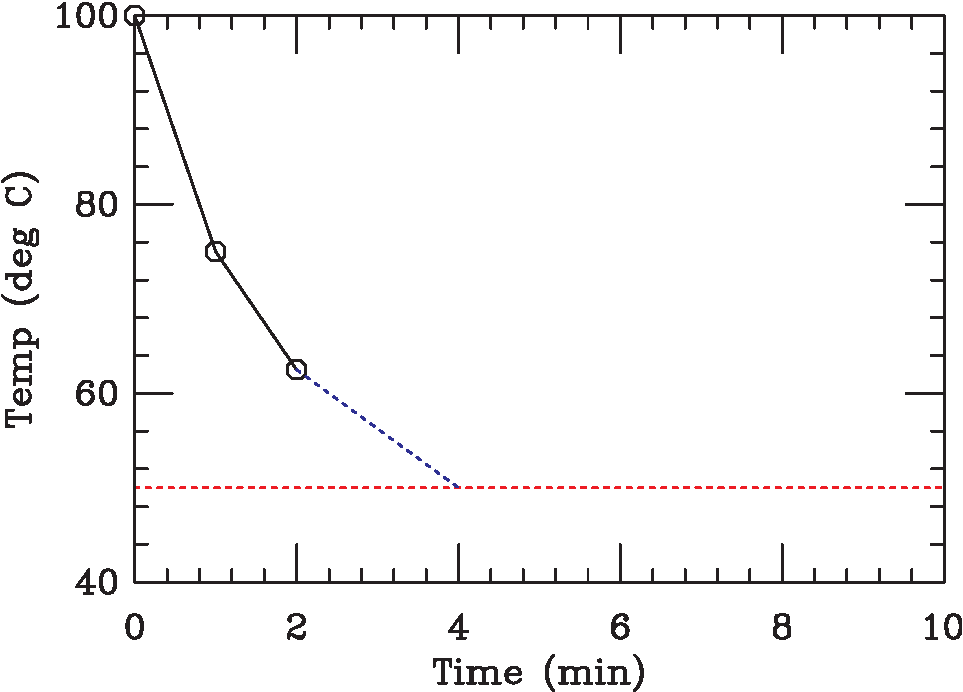
\includegraphics[width=0.9\textwidth]{fig2-crop.pdf}
\end{minipage}
\begin{minipage}{0.5\textwidth}
\begin{tabular}{|c | c | c |}
\hline
Time (min) & Temp (C) & Slope: $\PAR{T}{t}$ \\
\hline
0 & 100 & -25 \\
\hline
1 & 75 &  -12.5\\
\hline
2 & 62.5& -6.25 \\
\hline
3 & &  \\
\hline
4 & &  \\
\hline
5 & &  \\
\hline
\end{tabular}
\end{minipage}


\begin{minipage}{0.5\textwidth}
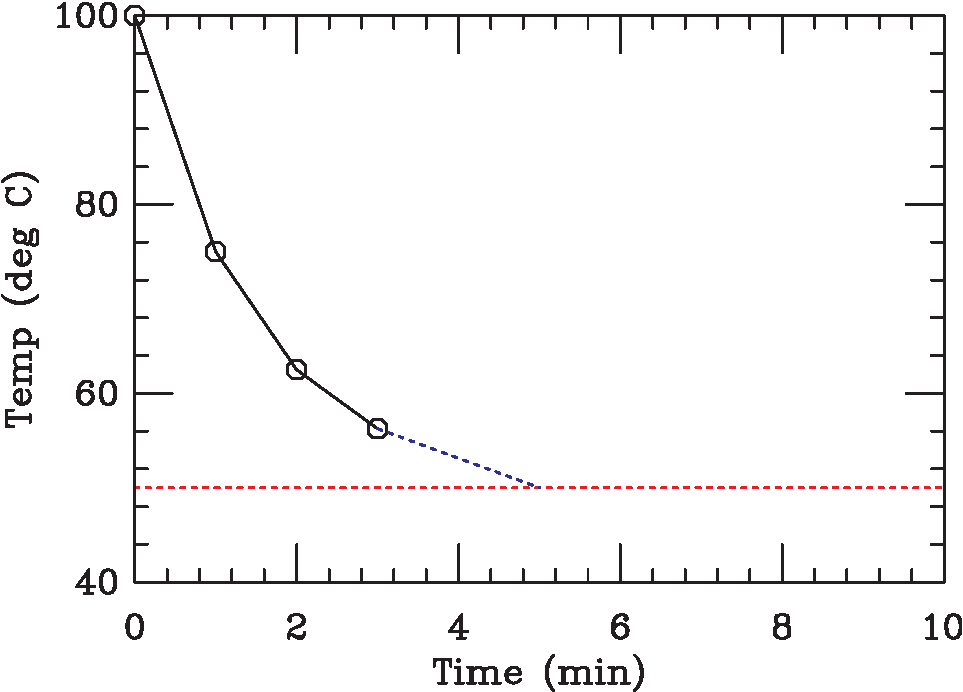
\includegraphics[width=0.9\textwidth]{fig3-crop.pdf}
\end{minipage}
\begin{minipage}{0.5\textwidth}
\begin{tabular}{|c | c | c |}
\hline
Time (min) & Temp (C) & Slope: $\PAR{T}{t}$ \\
\hline
0 & 100 & -25 \\
\hline
1 & 75 &  -12.5\\
\hline
2 & 62.5 & -6.25  \\
\hline
3 & 56.25 & -3.125 \\
\hline
4 & &  \\
\hline
5 & &  \\
\hline
\end{tabular}
\end{minipage}

And taking two more steps:

\begin{minipage}{0.5\textwidth}
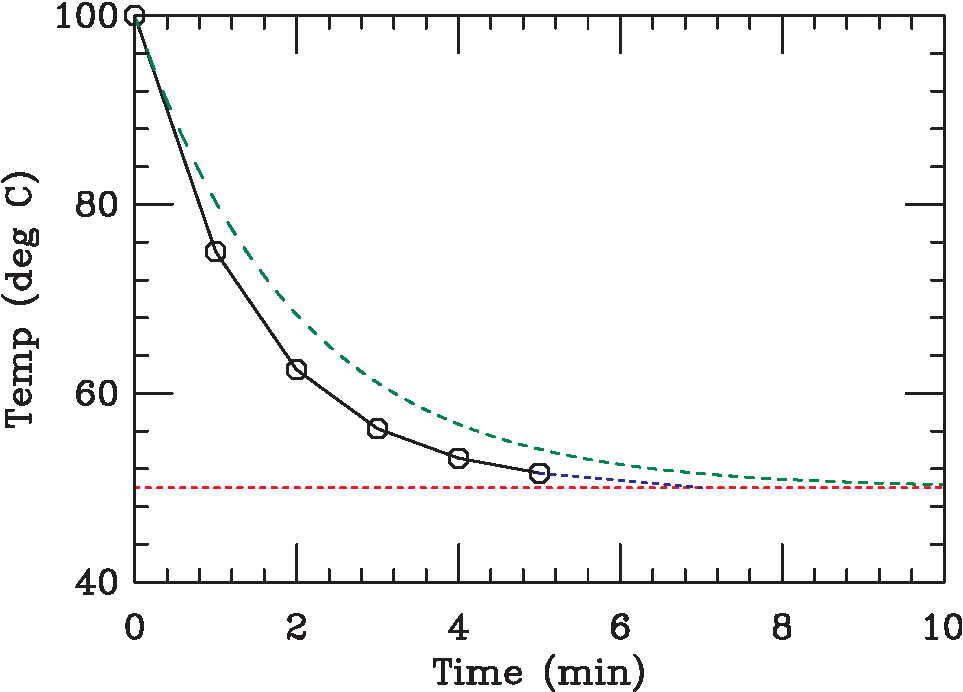
\includegraphics[width=0.9\textwidth]{fig5-crop.pdf}
\end{minipage}
\begin{minipage}{0.5\textwidth}
\begin{tabular}{|c | c | c |}
\hline
Time (min) & Temp (C) & Slope: $\PAR{T}{t}$ \\
\hline
0 & 100 & -25 \\
\hline
1 & 75 &  -12.5\\
\hline
2 & 62.5 & -6.25  \\
\hline
3 & 56.25 & -3.125 \\
\hline
4 & 53.125& -1.5625 \\
\hline
5 & 51.5625& 0.78125 \\
\hline
\end{tabular}
\end{minipage}

This last figure also shows the ``exact'' solution. What has gone wrong? You can
probably guess: during that first minute, we used a cooling rate of 25 degrees
per minute. However, as the tea cools, its cooling rate goes down: it wasn't 
25 deg/min for that {\it entire} time, only at the very start. You probably
have two ideas for what I should do:

\begin{itemize}
\item Use smaller steps
\item Do something akin to the midpoint rule
\end{itemize}

We'll talk about the equivalent to the midpoint rule later. Smaller steps help, as
you might expect. Here I'm using a step of 0.5 minute on the left, 
and 1 minute on the right:

\begin{minipage}{0.5\textwidth}
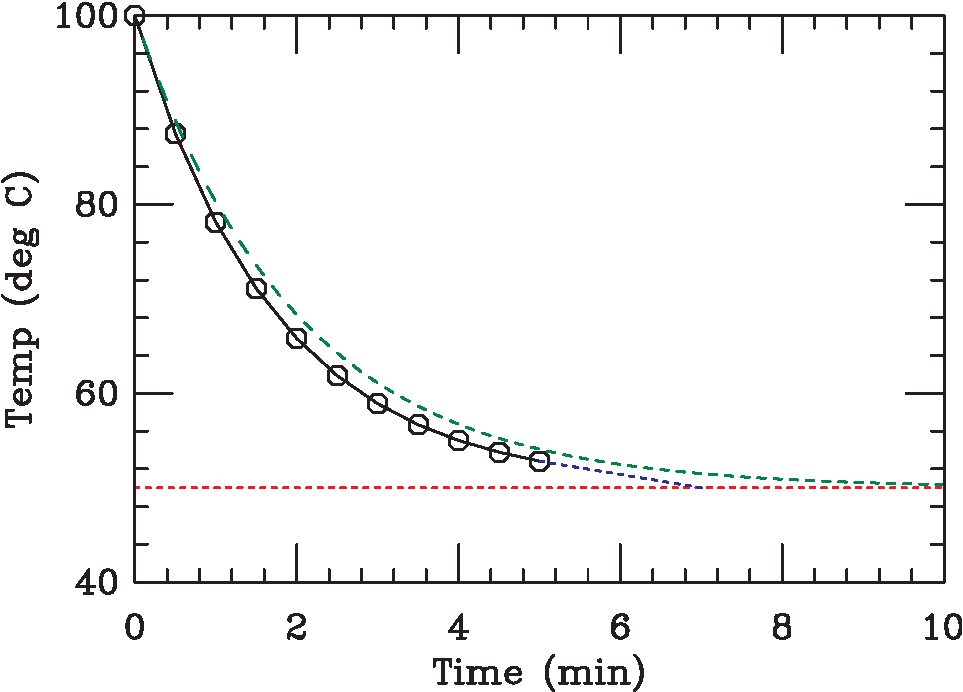
\includegraphics[width=0.9\textwidth]{figbetter-crop.pdf}
\end{minipage}
\begin{minipage}{0.5\textwidth}
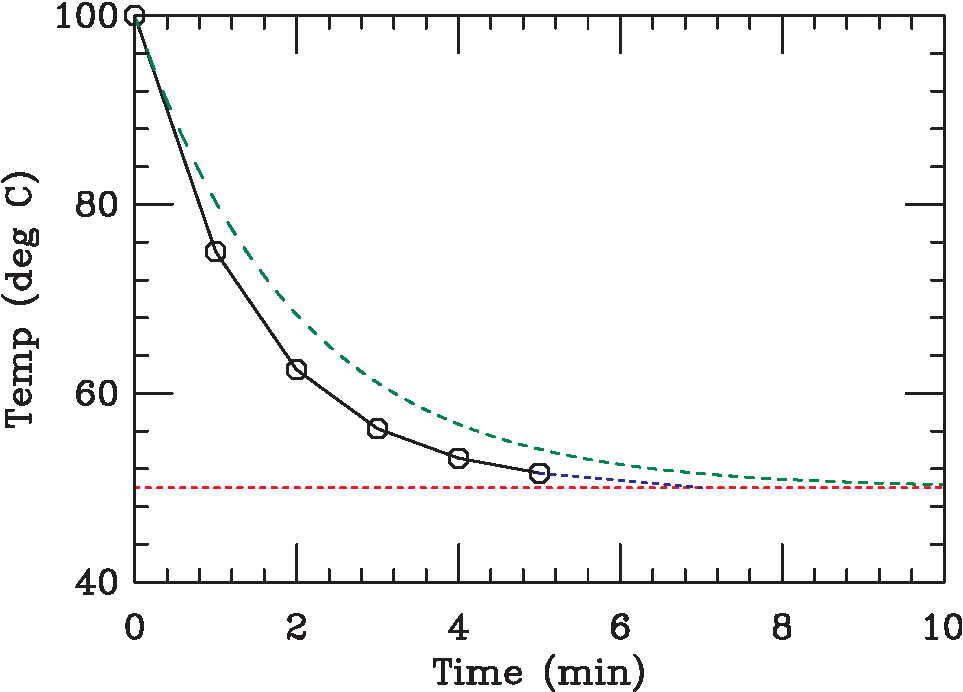
\includegraphics[width=0.9\textwidth]{fig5-crop.pdf}
\end{minipage}

You can see by eye that the error here is smaller.

The Euler method consists of doing the simplest thing you can think of: you approximate the value of the function at the end of each timestep by its value at the beginning, plus 
the rate of change times the length. In symbols,

\begin{equation}
  y(t+h) = y(t) + h f\left[y\left(t\right)\right];
\end{equation}

that is, the value after a timestep is equal to the value before the step, plus the length of the step times the rate of change. Since we need a value of $y$ to evaluate the rate
of change, we use the value at the beginning of the interval $y(t)$. For instance, for Newton's law of cooling, $f(T) = -k(T-T_a)$, and Euler's algorithm is

\begin{equation}
  T(t+h) = T(t) - hk(T-T_a) 
\end{equation}

Since this uses a left-hand-rule-type approach (estimate the slope during 
the interval using its value at the beginning), This is a ``first-order'' algorithm.

You've now learned how to solve first-order differential equations (here 
``first-order'' means that the DE includes only first derivatives, as 
opposed to ``first-order'' in the previous sentence -- damn mathematicians!).

We now have two possible next steps:

\begin{itemize}
\item Learn how to do something like the midpoint rule, to get better accuracy
for a given timestep
\item Learn how to handle second-order differential equations, like Newton's 
second law
\end{itemize}

You can learn about those in any order; I'll introduce the midpoint-like algorithm 
first.

\section{The RK2 algorithm}

The RK2 algorithm is analogous to the midpoint rule. Here, we would like to use the function's slope {\it halfway through the interval}, rather than at the beginning. We'd like to do something like this:

\begin{equation}
  y(t+h) = y(t) + h f\left[y\left(t+\frac{h}{2}\right)\right];
\end{equation}

The only trouble is that we don't know $y\left(t+\frac{h}{2}\right)$ -- in the Newton's law of cooling example, the temperature halfway through the interval. However, we can estimate it using the Euler method:

\begin{equation}
  y(t+\frac{h}{2}) = y(t) + \frac{h}{2} f\left[y\left(t\right)\right];
\end{equation}

This gives the following procedure for RK2:

\begin{enumerate}

  \item{Take an Euler-method half step to estimate the value of the variable $y$ at $t+h/2$}
  \item{Use that value $y(t+h/2)$ to compute the slope over the whole interval, and take a full step using that slope}
\end{enumerate}

In symbols, we have

\begin{align}
  y\left(t+\frac{h}{2}\right) =& y(t) + \frac{h}{2} f\left[y\left(t\right)\right] \\
  y(t+h) =& y(t) + h f\left[y\left(t+\frac{h}{2}\right)\right]
\end{align}

Let me now illustrate this in pictures, using $dt=1$ minute. Our procedure is:

\begin{itemize}
\item Use the temperature we know at (at $(t=0,T=100)$ to compute the slope there
\item Follow that slope out for a time interval equal to $dt/2$ (half a minute)
to get an estimate of the temperature at $t=0.5$ minute, the midpoint of the 
interval
\item Use this estimate of the temperature at 0.5 minute to compute an estimate
of the slope during the whole interval. This uses the same logic as the midpoint
rule: ``the average slope during the interval'' (the thing we want) is well-estimated
by ``the slope at the midpoint of the interval''.
\item Based on that estimate of the slope, starting with {\it the original
temperature value at the beginning of the interval}, figure out the temperature
at the end.
\item Repeat until golden brown around the edges.
\end{itemize}


\begin{minipage}{0.5\textwidth}
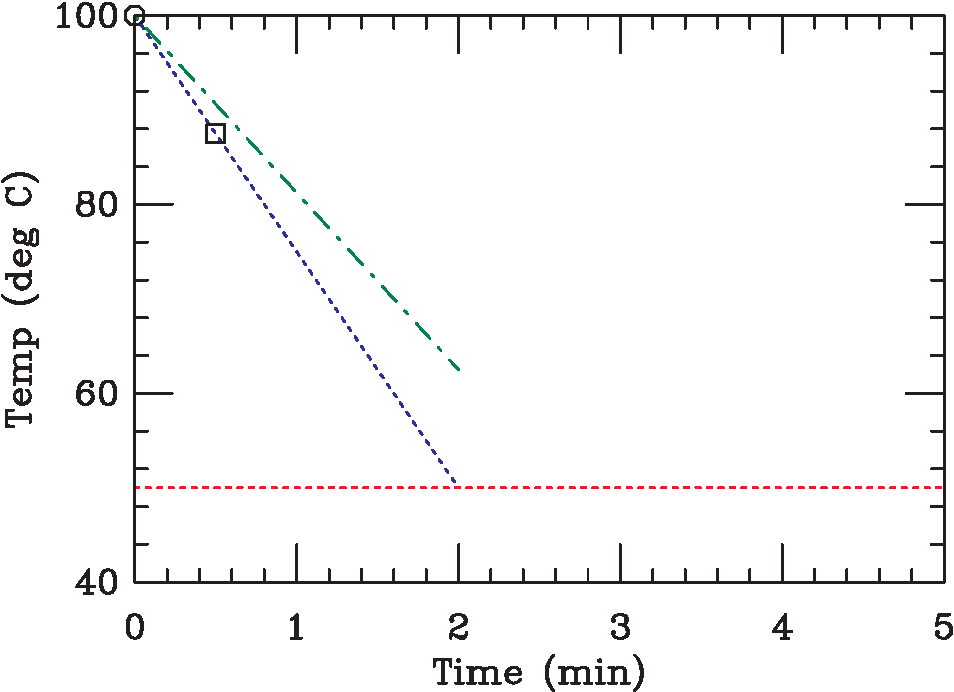
\includegraphics[width=0.9\textwidth]{rk0-crop.pdf}
\end{minipage}
\begin{minipage}{0.5\textwidth}
\begin{itemize}
\item The circle is the point we started with
\item The blue dotted line is the estimate of the slope at that temperature, $T(0)$
\item The square is the estimate of the temperature halfway through the step, $T_{\rm half}$
\item The green dashed line is the revised estimate of the slope during the 
interval, based on the value of $T_{\rm half}$.
\end{itemize}
\end{minipage}

Now, this is where we are:

\begin{minipage}{0.5\textwidth}
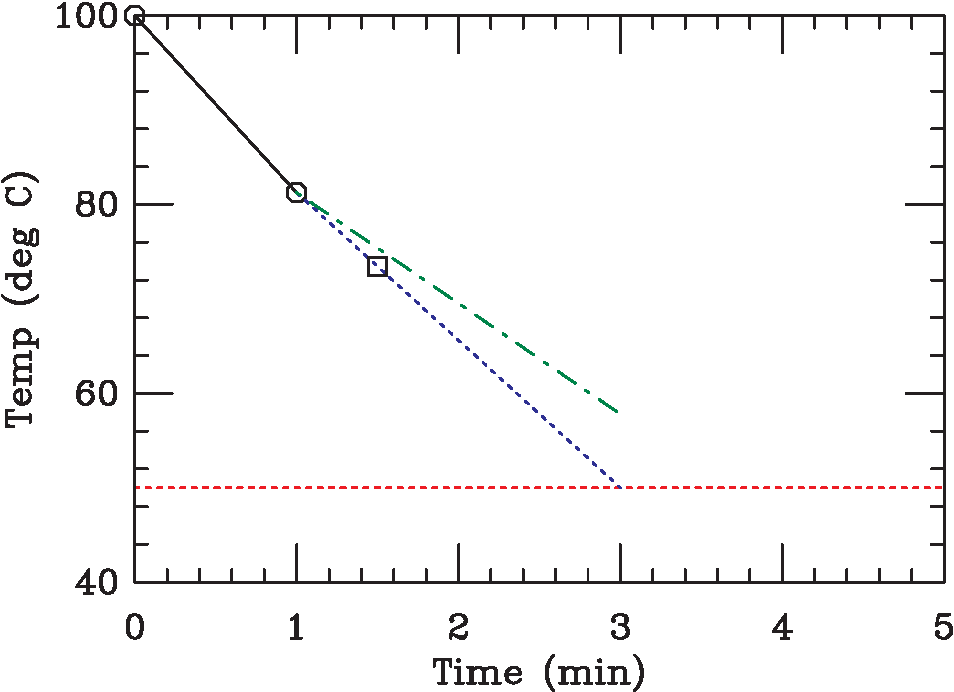
\includegraphics[width=0.9\textwidth]{rk1-crop.pdf}
\end{minipage}
\begin{minipage}{0.5\textwidth}
\begin{itemize}
\item Important: notice that the first step is taken starting from the 
{\it beginning} value -- the point $(0, 100)$ -- rather than the halfway estimate.
The halfway estimate is used {\it only} to estimate the slope used for the full
step, and then forgotten. 
\item The black line represents the first full step (which becomes part of our
solution). The blue dotted line is the slope estimate at $T(1)$, used to calculate
an estimate for the next value of $T_{\rm half}$; the green dashed line is the
estimate of the slope based on {\it that} temperature, which we will use for the 
third step...
\end{itemize}
\end{minipage}


\begin{minipage}{0.5\textwidth}
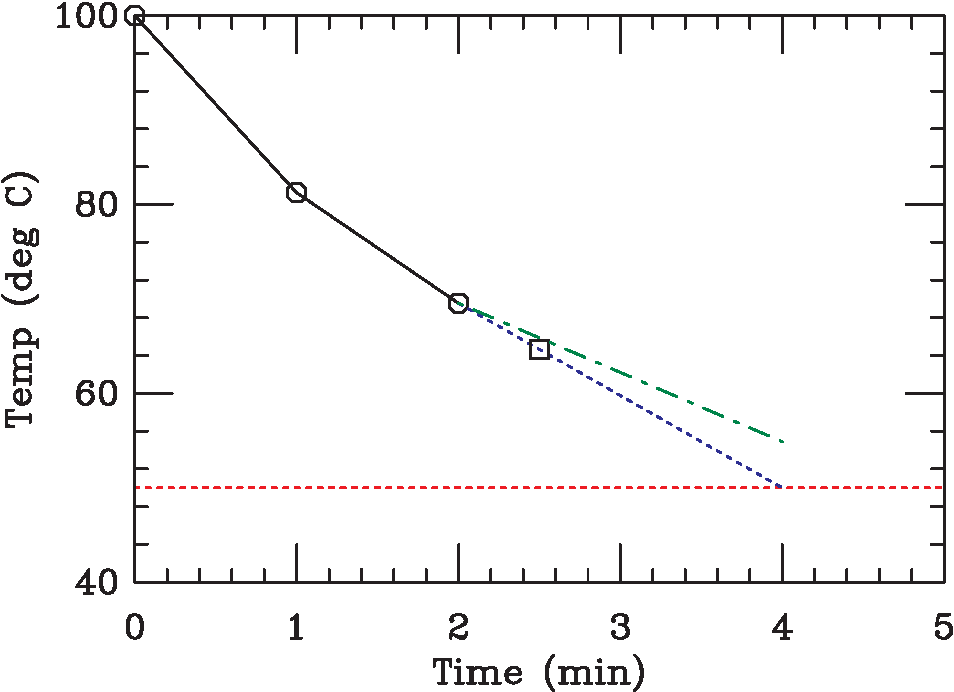
\includegraphics[width=0.9\textwidth]{rk2-crop.pdf}
\end{minipage}
\begin{minipage}{0.5\textwidth}
\begin{itemize}
\item ... and so on.
\end{itemize}
\end{minipage}

Comparing this RK2 method to Euler's method shows how much more accurate it is
for the same stepsize:

\begin{minipage}{0.5\textwidth}
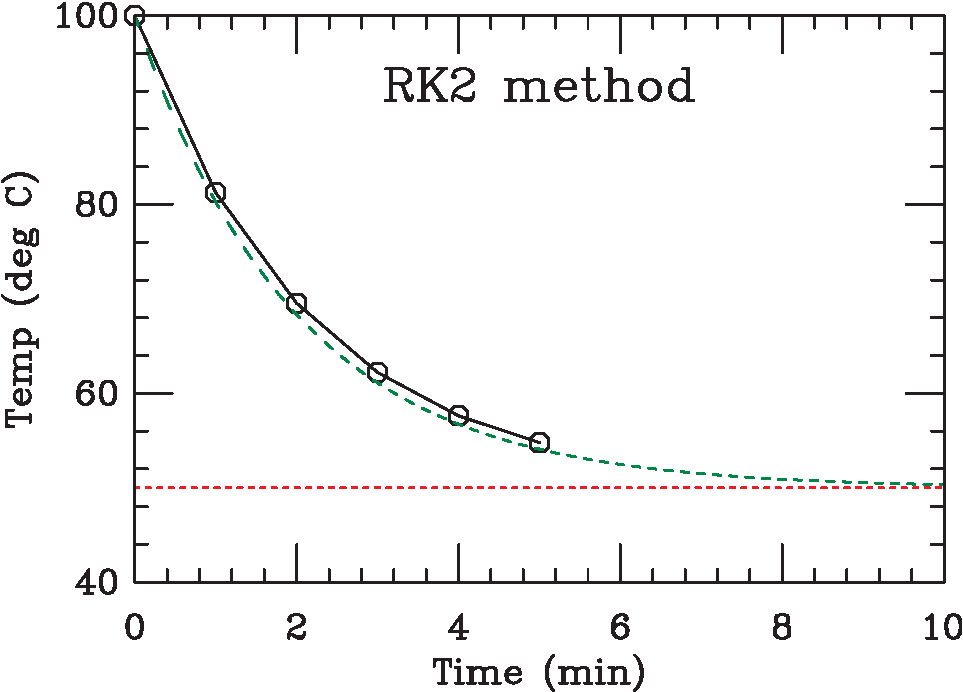
\includegraphics[width=0.9\textwidth]{rk5-crop.pdf}
\end{minipage}
\begin{minipage}{0.5\textwidth}
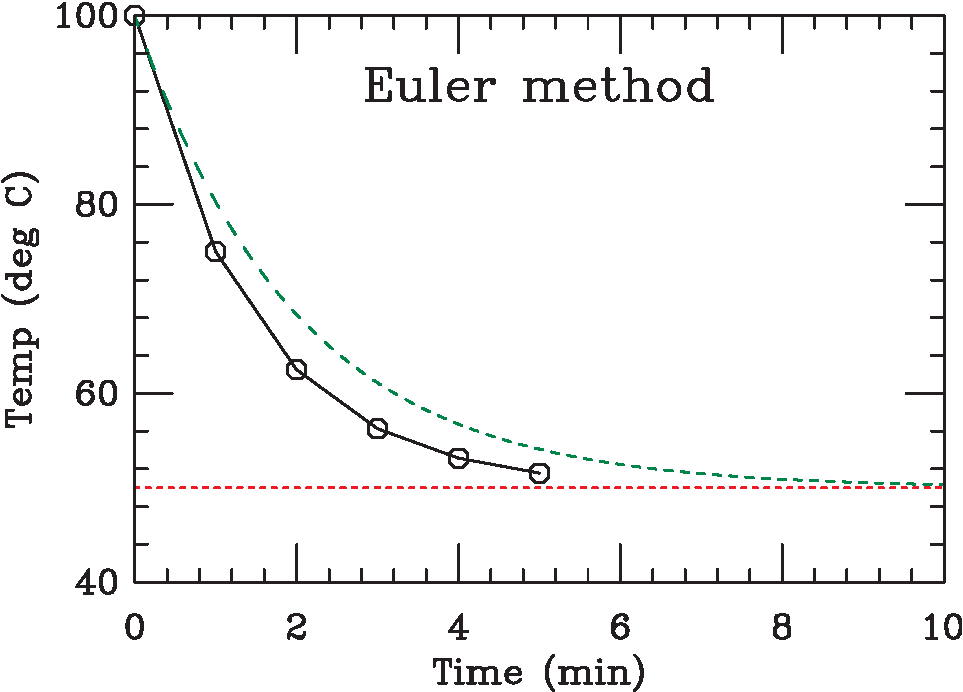
\includegraphics[width=0.9\textwidth]{euler5-crop.pdf}
\end{minipage}
\
\section{Euler's method for a single second-order DE}

A second-order differential equation can be reduced to two first-order DE's. In general, given the second-order differential equation

\begin{equation}
  \PARTWO{y}{t}=f(y)
\end{equation}

we can separate it into two {\it first-order DE's}:

\begin{align}
  \PAR {y}{t} =& \dot y \\
  \PAR {\dot y}{t} =& f(y,\dot y)
\end{align}

at the cost of introducing an extra {\it dynamical variable} $\dot y$. Dynamical variables are simply those variables that the simulation is evolving through time -- for instance, positions and velocities.

Then you do a straightforward Euler update for each:

\begin{align}
  y(t+h) =& y(t) + h \dot y(t) \\
  \dot y(t+h) =& \dot y(t) + h f\left[y(t),\dot y(t)\right]
\end{align}

As an example, for the swinging pendulum in your homework we have

\begin{align}
  \PAR{\theta}{t} =& \omega \\
  \PAR{\omega}{t} =& -g/L \sin \theta
\end{align}

and the Euler update looks like

\begin{align}
  \theta_{new} =& \theta_{old} + h \omega_{old} \\
  \omega_{new} =& \omega_{old} + h \frac{g}{L} \sin \theta_{old} \\
\end{align}

where I have used some new notation that should be easy to figure out.


\section{RK2 for a single second-order DE}

The approach here is just the same. The only trick is that you must take {\it both} half-steps together, since you need both $y$ and $\dot y$ evaluated at the halfway point to take the full step. The algorithm can be written

  \begin{align*}
    y\left(t+h/2\right) =& y(t) + \frac{h}{2} \dot y(t) \\
    \dot y\left(t+h/2\right) =& \dot y(t) + \frac{h}{2} f\left[y(t),\dot y(t)\right] \\
    y(t+h) =& y(t) + h \dot y(t+h/2) \\
   \dot y(t+h) =& \dot y(t) + h f\left[y\left(t+h/2\right),\dot y\left(t+h/2\right)\right]
  \end{align*}

For the pendulum in particular, our $y$ is the angle $\theta$ and $\dot y$ is the angular velocity $\omega$. Thus we have:

\begin{align*}
  \theta_{1/2} =& \theta_{old} + \frac{h}{2} \omega_{old} \\
  \omega_{1/2} =& \omega_{old} - \frac{h}{2} \frac{g}{L} \sin \theta_{old} \\
  \theta_{new} =& \theta_{old} + h \omega_{1/2} \\
  \omega_{new} =& \omega_{old} - h \frac{g}{L} \sin \theta_{1/2} \\
\end{align*}

  
\section{Euler's method for a system of many DE's}

In general, a large system of DE's with $N$ dynamical variables (which may be a combination of velocities and positions, as in the previous example, or may be something else) may be written

\begin{align*}
  \PAR{y_1}{t} =& f_1(y_1,y_2,y_3,y_4...)\\
  \PAR{y_2}{t} =& f_2(y_1,y_2,y_3,y_4...)\\
  \PAR{y_3}{t} =& f_3(y_1,y_2,y_3,y_4...)\\
  \PAR{y_4}{t} =& f_4(y_1,y_2,y_3,y_4...),
\end{align*}

where each rate of change $f_i$ depends on {\it all} of the dynamical variables $y_i$. In compact vector form, we can represent the vector of dynamical variables as $\vec y$ and their rates of change as $\vec f(\vec y)$. 
This is a vector function (it gives us a rate of change for each $y_i$) which has a vector parameter (it needs the value of all $y_i$'s). Then the collection of DE's can be written simply as 

\begin{equation}
  \PAR{\vec y}{t} = \vec f(\vec y)
\end{equation}

and the Euler algorithm becomes

\begin{equation}
  \vec y(t+h) = \vec y(t) + h \vec f\left[\vec y\left(t\right)\right];
\end{equation}

Note that all I did here is put vector signs over everything. It is easiest to understand how these algorithms work if you think of your collection of dynamical variables as a single object, and 
perform any operations on all of them at once. For HW4, for instance, you have four of them.

\section {RK2 for a system of many DE's}

You should already be able to guess how this goes: this is the same as RK2 for a single variable, except now we think about updating an entire {\it set} (which I've written as $\vec y$)  of dynamical variables. Some of these may be position variables 
(in which case their rate of change is a corresponding velocity variable), and some may be velocity variables (in which case their rates of change are given by Newton's second law), but it doesn't matter; the procedure is just ``do a half-step
for everything to get the values at the midpoint, and then use those values to do a full step''. 

We can write this in vector form as follows:

\begin{align}
    \vec y(t+\frac{h}{2}) =& \vec y(t) + \frac{h}{2} \vec f\left[\vec y\left(t\right)\right] \\
    \vec y(t+h) =& \vec y(t) + h \vec f\left[\vec y\left(t+\frac{h}{2}\right)\right]
\end{align}

where I have just scribbled vector signs above all the $y$'s and $h$'s that appeared in the one-equation RK2. It really is the same -- you just need to update a set of variables, rather than just one.

\section{Orbits around a fixed star}

Since planets orbit in a plane, we can restrict ourselves to the $x-y$ plane. This means we need four dynamical variables: $x, y, v_x, and v_y$. Let's put the Sun at the origin; then our variables tell us the position and velocity 
of the planet. We are going to have the set of DE's

\begin{align}
  \dot x =& v_x \\
  \dot y =& v_y \\
  \dot v_x =& a_x \\
  \dot v_y =& a_y \\
\end{align}

Now we just need to figure out what $a_x$ and $a_y$ are.

Newton's law of gravity tells us

\begin{equation}
  \vec F_g = (-\hat r) \frac{GMm}{r^2}
\end{equation}

where $\hat r$ is a unit vector pointing from the Sun to the planet, $M$ is the mass of the Sun, and $m$ is the mass of the planet. To compute the acceleration due to this force, we can use Newton's second law, which gives us

\begin{equation}
  m \vec a = (-\hat r) \frac{GMm}{r^2} \rightarrow \vec a = (-\hat r) \frac{GM}{r^2}
\end{equation}

Since we will be working in Cartesian coordinates, we need to find the $xi$ and $y-$ components of $\vec a$. This is done readily with the $\hat r-$trick. Note that

\begin{equation}
  \hat r = \frac{\vec r}{|r|}.
\end{equation}

This makes sense: $\hat r$ is a vector in the direction of $r$, but with length 1, so we just take $\vec r$ and divide it by its length $|r|$. Going forward I will drop the absolute value signs: $r \equiv |r| = \sqrt{x^2+y^2}$.
Now we convert everything into x and y components:

\begin{align}
  \vec r_x &= x \\
  \vec r_y &= y \\
  \hat r_x &= \frac{x}{r} \\
  \hat r_y &= \frac{y}{r} \\
  r &= \sqrt{x^2+y^2}
\end{align}

We can substitute this into Newton's law of gravity to get the $x$ and $y$ coordinates of the acceleration, which are what we want:

\begin{align}
  \vec a =& (-\hat r) \frac{GM}{r^2} \\
  \vec a =& (-\vec r) \frac{GM}{r^3} \\
  a_x =& \frac{-GMx}{r^3} \\
  a_y =& \frac{-GMy}{r^3}
\end{align}

  where $r=\sqrt{x^2+y^2}$. This gives us what we need: four DE's that give the rates of change of our four dynamical variables:

  \begin{align}
      \dot x =& v_x \\
      \dot y =& v_y \\
    \dot v_x =& \frac{-GMx}{(x^2+y^2)^{\frac{3}{2}}}\\
    \dot v_y =& \frac{-GMy}{(x^2+y^2)^{\frac{3}{2}}}\\
  \end{align}

  \end{document}




